%%%%
% Modificación de una plantilla de Latex para adaptarla al castellano.
%%%

%%%%%%%%%%%%%%%%%%%%%%%%%%%%%%%%%%%%%%%%%
% Thin Sectioned Essay
% LaTeX Template
% Version 1.0 (3/8/13)
%
% This template has been downloaded from:
% http://www.LaTeXTemplates.com
%
% Original Author:
% Nicolas Diaz (nsdiaz@uc.cl) with extensive modifications by:
% Vel (vel@latextemplates.com)
%
% License:
% CC BY-NC-SA 3.0 (http://creativecommons.org/licenses/by-nc-sa/3.0/)
%
%%%%%%%%%%%%%%%%%%%%%%%%%%%%%%%%%%%%%%%%%

%----------------------------------------------------------------------------------------
%	PACKAGES AND OTHER DOCUMENT CONFIGURATIONS
%----------------------------------------------------------------------------------------

\documentclass[paper=a4, fontsize=11pt]{scrartcl} % A4 paper and 11pt font size

% ---- Entrada y salida de texto -----

\usepackage[T1]{fontenc} % Use 8-bit encoding that has 256 glyphs
\usepackage[utf8]{inputenc}

% ---- Idioma --------

\usepackage[spanish, es-tabla]{babel} % Selecciona el español para palabras introducidas automáticamente, p.ej. "septiembre" en la fecha y especifica que se use la palabra Tabla en vez de Cuadro

% ---- Otros paquetes ----

% Hipervínculos
\usepackage[hidelinks]{hyperref}

\usepackage{amsmath,amsfonts,amsthm} % Math packages
\usepackage{graphics,graphicx, float, url} %para incluir imágenes y colocarlas
% \usepackage{ulem}

\usepackage{fancyhdr} % Custom headers and footers
\pagestyle{fancyplain} % Makes all pages in the document conform to the custom headers and footers
\fancyhead{} % No page header - if you want one, create it in the same way as the footers below
\fancyfoot[L]{} % Empty left footer
\fancyfoot[C]{} % Empty center footer
\fancyfoot[R]{\thepage} % Page numbering for right footer
\renewcommand{\headrulewidth}{0pt} % Remove header underlines
\renewcommand{\footrulewidth}{0pt} % Remove footer underlines
\setlength{\headheight}{13.6pt} % Customize the height of the header

\numberwithin{equation}{section} % Number equations within sections (i.e. 1.1, 1.2, 2.1, 2.2 instead of 1, 2, 3, 4)
\numberwithin{figure}{section} % Number figures within sections (i.e. 1.1, 1.2, 2.1, 2.2 instead of 1, 2, 3, 4)
\numberwithin{table}{section} % Number tables within sections (i.e. 1.1, 1.2, 2.1, 2.2 instead of 1, 2, 3, 4)

\setlength\parindent{0pt} % Removes all indentation from paragraphs - comment this line for an assignment with lots of text

\newcommand{\horrule}[1]{\rule{\linewidth}{#1}} % Create horizontal rule command with 1 argument of height

%% Para incluir archivos en texto plano
\usepackage{listings}

%----------------------------------------------------------------------------------------
%	TITLE
%----------------------------------------------------------------------------------------

\title{\textbf{Benchmarks 103}\\ % Title
Testing Memory Benchmark} % Subtitle

\author{Óscar Bermúdez Garrido\\ \href{http://www.github.com/oxcar103}{@oxcar103} % Nombre y apellidos
\\{\textit{Universidad de Granada}}} % Institution

\date{\today} % Date

%----------------------------------------------------------------------------------------

\begin{document}

\maketitle % Print the title section

\tableofcontents

\pagebreak

	\section{Documentación del benchmark}
		Este benchmark realiza un análisis de velocidad de lectura y escritura en memoria, ya sea
		tanto de unidades internas como un disco duro o externas como una memoria USB.
		
		Para el correcto funcionamiento del benchmark, se requiere de su ejecución con los siguientes
		parámetros:
		
		\begin{itemize}
			\item \textbf{Tamaño}: El número de Gigabytes que se leerán/escribirán\footnote{Por el
			diseño del benchmark, es necesario que se tenga en el dispositivo al menos el doble de
			este valor libre, ya que para la prueba de lectura/escritura se necesitan 2 archivos
			simultáneamente. Estos archivos se borrarán al finalizar, siempre y cuando el programa
			termine su ejecución correctamente}.
			
			\item \textbf{Archivo}: El archivo de donde se sacarán los datos\footnote{En Linux, se
			recomienda usar \textit{/dev/urandom}.}.
			
			\item \textbf{Direcciones}: Las direcciones a los distintos dispositivos en los que se
			realizará la prueba. Mínimo: 1.
		\end{itemize}
		
		Para la medición del tiempo, se ha optado por la utilización de las instrucciones
		\textit{gettimeofday} y \textit{timersub}. Dado que \textit{gettimeofday} tiene un tiempo
		de ejecución del orden de las milésimas de segundo y se ejecuta justo al empezar y al
		terminar a \textsc{escribir}/\textsc{leer}/\textsc{leer-y-escribir}, y los resultados son
		del orden de los segundos(incluso de los minutos), no considero que afecte en gran cantidad
		a la medición.
		
	\section{Documentación del experimento}
		Construiremos un experimento con la finalidad de determinar si realmente la diferencia de
		velocidad entre dispositivos de almacenamiento interno y externo es tan grande como cabe
		pensar a priori y si el sistema de archivos repercute significativamente en la velocidad
		de acceso a los datos.
		
		Por ello, para el experimento, se utilizará mi disco duro, que contiene varias particiones,
		en concreto, la partición de \textit{Linux} con \textbf{ext4} y la partición de
		\textit{Windows} con \textbf{nfts} y una memoria externa, enconcreto, un pendrive USB.
		
		La prueba consiste en realizar 5 veces:
		
		\begin{itemize}
			\item Tomar 1 MB del archivo pasado, y copiar hasta obtener 1GB\footnote{Nótese que si
			copiamos el contenido en un array auxiliar, concatenamos y repetimos, tras 1024
			iteraciones ya tendremos 1 GB.}.
			
			\item Para cada dirección pasada como parámetro:
				\begin{itemize}
					\item Creamos 2 archivos.
			
					\item Escribimos tantos Gigabytes como indique el parámetro pasado de uno en
					uno Gigabyte\footnote{Yo pasaré 5GB como tamaño}.
			
					\item Leemos tantos Gigabytes como indique el parámetro pasado de uno en uno
					Gigabyte.
			
					\item Leemos del primer archivo y escribimos en el segundo tantos Gigabytes
					como indique el parámetro pasado de uno en uno Gigabyte.
								
					\item Eliminamos los archivos.
				\end{itemize}
		\end{itemize}
		
	\section{Resultados del experimento}
		Estos son los resultados:
		
		\lstinputlisting{Resultados.csv}
		
		\begin{figure}[H]
			\centering
			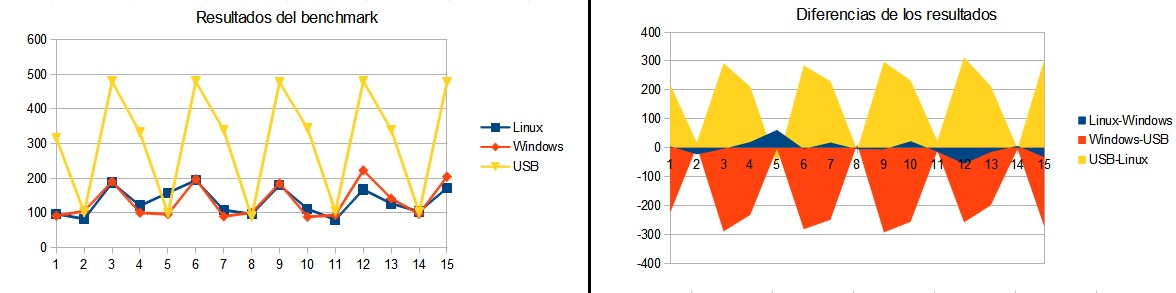
\includegraphics[width=15cm]{Graficas.jpg}
			\caption{Gráfica con los resultados del experimento con el benchmark.}
			\label{fig:graph}	
		\end{figure}
		
		Tras obtener los resultados del benchmark, realizamos el procedimiento visto en las clases
		de teoría, calculamos la \textit{media} y la \textit{desviación típica} de las diferencias y
		vemos si podrían pertenecer a una distribución \textit{T-Student} con $n-1$ grados de
		libertad, es decir, 14 grados de libertad.
		
		Como podemos ver en la figura, no obtenemos resultados significativos entre distintas
		versiones del sistema de ficheros pero sí entre el disco duro y la memoria USB, con una
		media de 170 segundos en cada fase de la prueba\footnote{Imagen tomada del archivo
		Resultados.ods}:
		 
		 \begin{figure}[H]
 			\centering
			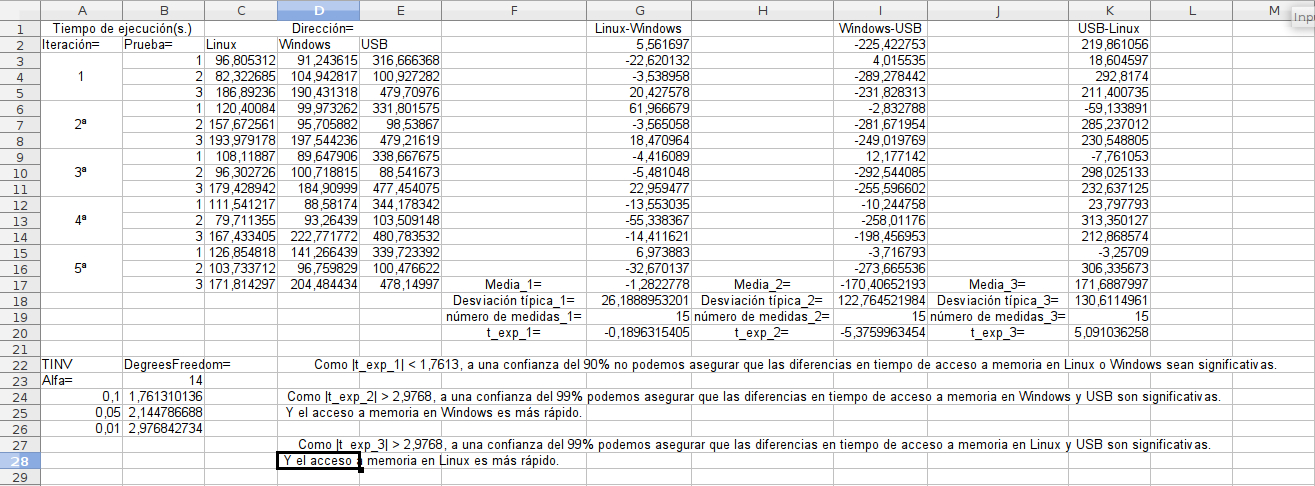
\includegraphics[width=15cm]{Resultados.jpg}
 			\caption{Resultados del experimento con el benchmark.}
 			\label{fig:benchmark}	
 		\end{figure}

		\cite{man_benchmark}

\newpage
\section{Referencias}
\begin{thebibliography}{10}
\expandafter\ifx\csname url\endcsname\relax
  \def\url#1{\texttt{#1}}\fi
\expandafter\ifx\csname urlprefix\endcsname\relax\def\urlprefix{URL}\fi
\expandafter\ifx\csname href\endcsname\relax
  \def\href#1#2{#2} \def\path#1{#1}\fi

\bibitem{man_benchmark}
Todos los manuales(o casi) de las instrucciones usadas en benchmark.c: \textit{strcpy}\cite{man_strcpy},
\textit{strcat}\cite{man_strcat}, \textit{fopen}\cite{man_fopen}, \textit{fclose}\cite{man_fclose},
\textit{fread}\cite{man_fread}, \textit{fwrite}\cite{man_fwrite}, \textit{fprintf}\cite{fprintf},
\textit{gettimeofday}\cite{man_gettimeofday} y \textit{timersub}\cite{man_timersub}.

\bibitem{man_strcpy}
Ubuntu manuals\\
strcpy(3) - Linux man page\\
  \url{http://manpages.ubuntu.com/manpages/xenial/en/man3/strcpy.3.html}

\bibitem{man_strcat}
Ubuntu manuals\\
strcat(3) - Linux man page\\
  \url{http://manpages.ubuntu.com/manpages/xenial/en/man3/strcat.3.html}

\bibitem{man_fopen}
Ubuntu manuals\\
fopen(3) - Linux man page\\
  \url{http://manpages.ubuntu.com/manpages/xenial/en/man3/fopen.3.html}

\bibitem{man_fclose}
Ubuntu manuals\\
fclose(3) - Linux man page\\
  \url{http://manpages.ubuntu.com/manpages/xenial/en/man3/fclose.3.html}

\bibitem{man_fread}
Ubuntu manuals\\
fread(3) - Linux man page\\
  \url{http://manpages.ubuntu.com/manpages/xenial/en/man3/fread.3.html}

\bibitem{man_fwrite}
Ubuntu manuals\\
fwrite(3) - Linux man page\\
  \url{http://manpages.ubuntu.com/manpages/xenial/en/man3/fwrite.3.html}

\bibitem{man_fprintf}
Ubuntu manuals\\
fprintf(3) - Linux man page\\
  \url{http://manpages.ubuntu.com/manpages/xenial/en/man3/fprintf.3.html}

\bibitem{man_gettimeofday}
Ubuntu manuals\\
gettimeofday(2) - Linux man page\\
  \url{http://manpages.ubuntu.com/manpages/xenial/en/man2/gettimeofday.2.html}

\bibitem{man_timersub}
Ubuntu manuals\\
timersub(3) - Linux man page\\
  \url{http://manpages.ubuntu.com/manpages/xenial/en/man3/timersub.3.html}

\end{thebibliography}

\end{document}